%#####################################################################
\chapter{ns-3によるOpenFlowネットワーク構築}
%#####################################################################

 本研究では,現在愛媛大学が採用しているEUNETを対象にした新たなネットワークシステムのモデルを提案する.
本章では,現在のシステムであるEUNETについて説明し,今回の研究で提案するOpenFlowを用いたネットワークモデルの構築法について説明する.

\section{EUNET}

現在,愛媛大学ではEUNETと呼ばれるネットワークが稼働している.
EUNETは大きく分けると,キャンパス内を網羅するエッジネットワークと,愛媛大学の城北,重信,樽味,持田の各キャンパスとデータセンタを接続するL3サブネットの二種類があり,EUNET全体で現時点で約700ものネットワーク機器を用いて運営されている.

\subsubsection{L3サブネット}

EUNETの中心部に位置するネットワーク.
愛媛大学の各キャンパス及びデータセンタに設置されているコアスイッチ群,以下に説明するスーパーコアから構成され,愛媛大学の各キャンパス間の接続およびインターネットとの接続を行う.

\subsubsection{スーパーコア}

L3サブネットの中核を成すネットワーク機器群.
EUNETとインターネットとの接続点に設置されており,ファイアウォール,検疫ゲートウェイ,侵入防止システム(IPS),セキュアゲートウェイの機能を持ち,EUNETに悪影響を与える可能性のある通信について対処する機能を備える.
インターネットなど外部との接続の場合のみならず,EUNET内部でも異なるセグメント間の通信は,必ずスーパーコアを通るような設計になっており,ネットワーク内部の脅威にも対応することが可能である.

しかし,現在のスーパーコアの設計は,異なるセグメント間の通信を通す際に,図 \ref{fig:3-0}のような経路選択のもと,通信を行っている.
このような構造の場合,通常のインラインモードのIPSでは正常に動作が保証されておらず,限られたごく僅かなIPSでしか動作しない.
事実として,現在導入されているIPSはこのスーパーコアを正常に稼働させられる唯一のIPSであり,もしこのIPSの製造が行われなくなった場合,スーパーコアの設計の変更を余儀なくされる可能性がある.

\begin{figure}[tb]
	\begin{center}
		\scalebox{0.5}{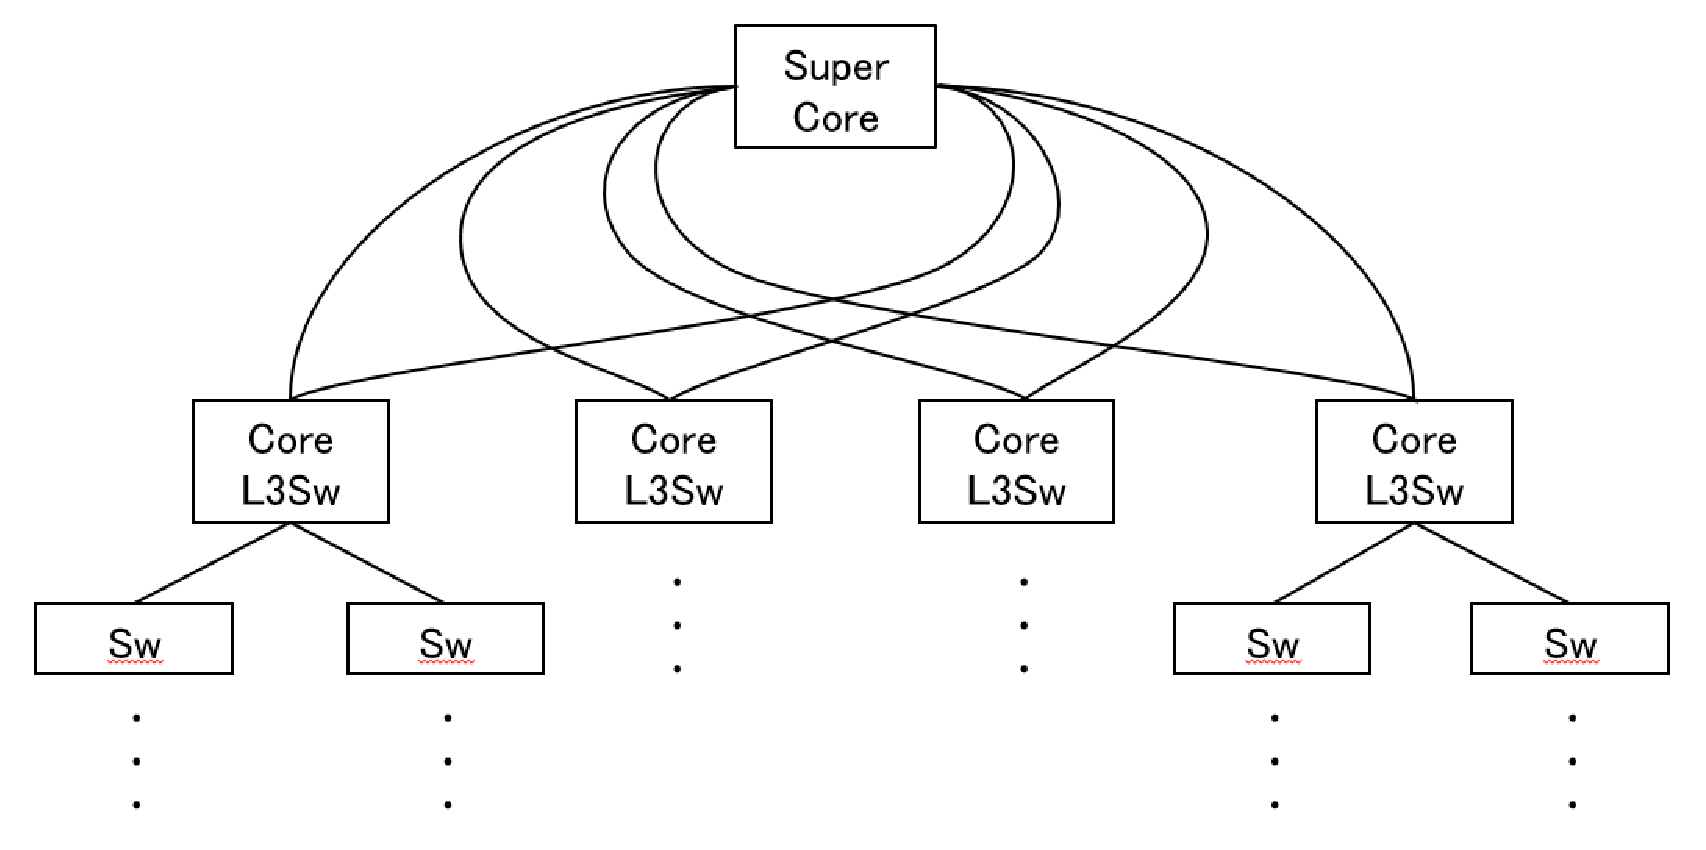
\includegraphics{./img/eps/3-0.eps}} 
		\caption{現在のスーパーコアの設計}
		\label{fig:3-0}
	\end{center}
\end{figure}

\section{ネットワークモデル構築法}

本節では,上記の問題点があるスーパーコアを設計に手を加える形となった本研究のネットワークモデルを構築するための方法を説明する.
本研究で製作するネットワークモデルを用いた場合,2.3節で述べたIPS機のほぼ全てで従来と同様のセキュリティ機能が期待される.

本研究では,スーパーコア周辺のパケットの制御に関する提案を行っているため,スーパーコアを問題なくパケットが通過するかをわかりやすく判断するために,すべてのパケット通信をスーパーコアに一度経由させることとする.
スイッチをOpenFlow対応スイッチへと変更してネットワークを構成し,2種類のOpenFlowコントローラによってスイッチを制御することで,図 \ref{fig:3-1}のようなネットワークを構築する.
OpenFlowスイッチは,次に説明する2種類のOpenFlowコントローラによって制御を行う.

\begin{figure}[tb]
	\begin{center}
		\scalebox{0.5}{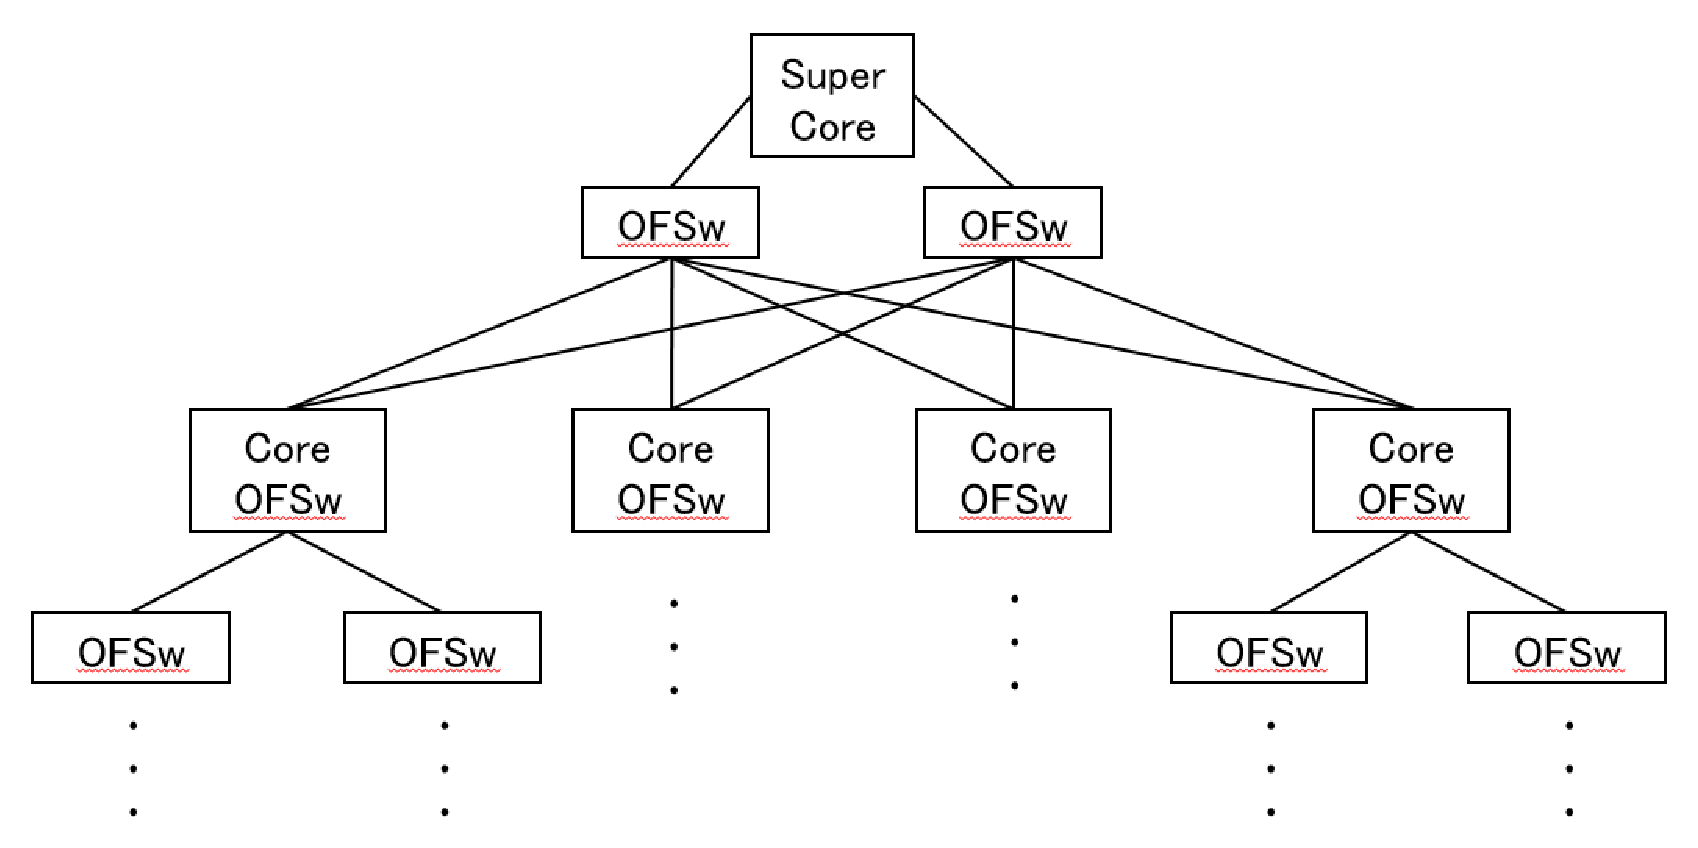
\includegraphics{./img/eps/3-1.eps}} 
		\caption{提案するネットワークモデル}
		\label{fig:3-1}
	\end{center}
\end{figure}

\subsubsection{BasicController}

BasicControllerは,コアスイッチより下層に位置するスイッチ全て,および従来のスーパーコアとコアスイッチの間に新たに設置するスイッチを制御するOpenFlowコントローラである.
所属するOpenFlowスイッチは,物理ポートの1つを上層のネットワークと接続し,それ以外の物理ポートを下層のネットワークおよびホストと接続させることが必要.
下層のネットワークおよびホストから入力されたパケットを無条件で上層のネットワークへと出力し,上層のネットワークから入力されたパケットは,経路規則に従い下層のネットワークおよびホストへと出力するという処理を行う.

\subsubsection{CoreSwitchController}

CoreSwitchControllerは,コアスイッチを制御するOpenFlowコントローラである.
コアスイッチは,物理ポート2つをスーパーコアとコアスイッチの間に新たに設置するスイッチ2つにそれぞれ接続し,それ以外の物理ポートを下層のネットワークと接続させる.

下層のネットワークから入力されたパケットは,上層のネットワークへ出力する際に,MACアドレスの比較を用いて出力する物理ポートを決定する.
パケットから送信元MACアドレスと宛先MACアドレスを取り出し,送信元MACアドレスの方が小さい場合は物理ポート0から,大きい場合は物理ポート1から出力するように処理を行う.
このとき,コアスイッチの物理ポート0から出力されたパケットはスーパーコアの物理ポート0から入力されるように,物理ポート1から出力されたパケットは物理ポート1から入力されるように結線を行われている.
MACアドレスは各ネットワーク機器に対して,唯一かつ一意に割り振られているため,通信を行う任意のホスト2台間の通信経路は一意に決定され,通信の対称性が保証される.

上層のネットワークから入力されたパケットは,経路規則に従い出力ポートを決定する.
このとき,上層のネットワークに出力しないように設定する必要がある.